%
% ---------------------------------------------------------------
% Copyright (C) 2012-2018 Gang Li
% ---------------------------------------------------------------
%
% This work is the default powerdot-tuliplab style test file and may be
% distributed and/or modified under the conditions of the LaTeX Project Public
% License, either version 1.3 of this license or (at your option) any later
% version. The latest version of this license is in
% http://www.latex-project.org/lppl.txt and version 1.3 or later is part of all
% distributions of LaTeX version 2003/12/01 or later.
%
% This work has the LPPL maintenance status "maintained".
%
% This Current Maintainer of this work is Gang Li.
%
%

\documentclass[
 size=14pt,
 paper=smartboard,  %a4paper, smartboard, screen
 mode=present, 		%present, handout, print
 display=slides, 	% slidesnotes, notes, slides
 style=tuliplab,  	% TULIP Lab style
 pauseslide,
 fleqn,leqno]{powerdot}


\usepackage{cancel}
\usepackage{caption}
\usepackage{stackengine}
\usepackage{smartdiagram}
\usepackage{attrib}
\usepackage{amssymb}
\usepackage{amsmath} 
\usepackage{amsthm} 
\usepackage{mathtools}
\usepackage{rotating}
\usepackage{graphicx}
\usepackage{boxedminipage}
\usepackage{rotate}
\usepackage{calc}
\usepackage[absolute]{textpos}
\usepackage{psfrag,overpic}
\usepackage{fouriernc}
\usepackage{pstricks,pst-3d,pst-grad,pstricks-add,pst-text,pst-node,pst-tree}
\usepackage{moreverb,epsfig,subfigure}
\usepackage{color}
\usepackage{booktabs}
\usepackage{etex}
\usepackage{breqn}
\usepackage{multirow}
\usepackage{natbib}
\usepackage{bibentry}
\usepackage{gitinfo2}
\usepackage{siunitx}
\usepackage{nicefrac}
%\usepackage{geometry}
%\geometry{verbose,letterpaper}
\usepackage{media9}
\usepackage{animate}
%\usepackage{movie15}
\usepackage{auto-pst-pdf}

\usepackage{breakurl}
\usepackage{fontawesome}
\usepackage{xcolor}
\usepackage{multicol}



\usepackage{verbatim}
\usepackage[utf8]{inputenc}
\usepackage{dtk-logos}
\usepackage{tikz}
\usepackage{adigraph}
%\usepackage{tkz-graph}
\usepackage{hyperref}
%\usepackage{ulem}
\usepackage{pgfplots}
\usepackage{verbatim}
\usepackage{fontawesome}


\usepackage{todonotes}
% \usepackage{pst-rel-points}
\usepackage{animate}
\usepackage{fontawesome}

\usepackage{listings}
\lstset{frameround=fttt,
frame=trBL,
stringstyle=\ttfamily,
backgroundcolor=\color{yellow!20},
basicstyle=\footnotesize\ttfamily}
\lstnewenvironment{code}{
\lstset{frame=single,escapeinside=`',
backgroundcolor=\color{yellow!20},
basicstyle=\footnotesize\ttfamily}
}{}


\usepackage{hyperref}
\hypersetup{ % TODO: PDF meta Data
  pdftitle={Presentation Title},
  pdfauthor={Gang Li},
  pdfpagemode={FullScreen},
  pdfborder={0 0 0}
}


% \usepackage{auto-pst-pdf}
% package to show source code

\definecolor{LightGray}{rgb}{0.9,0.9,0.9}
\newlength{\pixel}\setlength\pixel{0.000714285714\slidewidth}
\setlength{\TPHorizModule}{\slidewidth}
\setlength{\TPVertModule}{\slideheight}
\newcommand\highlight[1]{\fbox{#1}}
\newcommand\icite[1]{{\footnotesize [#1]}}

\newcommand\twotonebox[2]{\fcolorbox{pdcolor2}{pdcolor2}
{#1\vphantom{#2}}\fcolorbox{pdcolor2}{white}{#2\vphantom{#1}}}
\newcommand\twotoneboxo[2]{\fcolorbox{pdcolor2}{pdcolor2}
{#1}\fcolorbox{pdcolor2}{white}{#2}}
\newcommand\vpspace[1]{\vphantom{\vspace{#1}}}
\newcommand\hpspace[1]{\hphantom{\hspace{#1}}}
\newcommand\COMMENT[1]{}

\newcommand\placepos[3]{\hbox to\z@{\kern#1
        \raisebox{-#2}[\z@][\z@]{#3}\hss}\ignorespaces}

\renewcommand{\baselinestretch}{1.2}


\newcommand{\draftnote}[3]{
	\todo[author=#2,color=#1!30,size=\footnotesize]{\textsf{#3}}	}
% TODO: add yourself here:
%
\newcommand{\gangli}[1]{\draftnote{blue}{GLi:}{#1}}
\newcommand{\shaoni}[1]{\draftnote{green}{sn:}{#1}}
\newcommand{\gliMarker}
	{\todo[author=GLi,size=\tiny,inline,color=blue!40]
	{Gang Li has worked up to here.}}
\newcommand{\snMarker}
	{\todo[author=Sn,size=\tiny,inline,color=green!40]
	{Shaoni has worked up to here.}}

%%%%%%%%%%%%%%%%%%%%%%%%%%%%%%%%%%%%%%%%%%%%%%%%%%%%%%%%%%%%%%%%%%%%%%%%
% title
% TODO: Customize to your Own Title, Name, Address
%
\title{What's Cooking}
\author{
Siyu Chen
\\
\\Xi'an Shiyou University

}
\date{\gitCommitterDate}


% Customize the setting of slides
\pdsetup{
% TODO: Customize the left footer, and right footer
rf=\href{http://www.tulip.org.au}{
Last Changed by: \textsc{\gitCommitterName}\ \gitVtagn-\gitAbbrevHash\ (\gitAuthorDate)
},
cf={What's Cooking},
}


\begin{document}

\maketitle

%\begin{slide}{Overview}
%\tableofcontents[content=sections]
%\end{slide}


%%==========================================================================================
%%
\begin{slide}[toc=,bm=]{Overview}
\tableofcontents[content=currentsection,type=1]
\end{slide}
%%
%%==========================================================================================


\section{Problem Definition}


%%==========================================================================================
%%
\begin{slide}{Problem Description}
\begin{center}
\twotonebox{\rotatebox{90}{Description}}{\parbox{.86\textwidth}
{Asks you to predict the category of a dish's cuisine given a list of its ingredients. 
\begin{itemize}
\item 1. Dish data loading;
\item 2. Preprocess seasoning and visualization data set structure;
\item 3. Loading Logistic Regression Model and Ensemble Model training;
\item 4. Test and submit the results to see the experimental score.
\end{itemize}
}}

\end{center}
\bigskip
\begin{center}
\end{center}
\bigskip

%%==========================================================================================
\begin{note}
First, I will introduce the problem definition.
In the real life,
a teacher may be interested in the characteristics that
make one student obvious different from others.
Or,
NBA sports coaches would prefer to
know the advantages and disadvantages of one player.
Here, the player can be regarded as a query object.

For example, team A has five players,
each player has four features.
The NBA sports coaches may want to know the features of
player $1$ that are different from others.

The above example can be seen as outlying aspects mining.
The main purpose of outlying aspects mining is to identify
the outstanding features of the query object.
\end{note}
%%==========================================================================================

\end{slide}
%%
%%==========================================================================================


%%==========================================================================================
%%
\begin{slide}[toc=,bm=]{Read Data}
\begin{center}

\end{center}

\bigskip

\twocolumn[
\savevalue{lfrheight}=8cm,
\savevalue{lfrprop}={
linestyle=solid,framearc=.2,linewidth=1pt},
rfrheight=\usevalue{lfrheight},
rfrprop=\usevalue{lfrprop}
]{
  
\begin{itemize}
\item
\smallskip
\textcolor{orange}{train.tsv} :The data used for training that contains ID, cuisine, and ingredients.
\smallskip
\item
\smallskip
\textcolor{orange}{test.tsv} : After training the model with the training data set, use the test data set to generate a file similar to sample_submission.csv.
\smallskip
\item
\smallskip
\textcolor{orange}{sampleSubmission.csv} : A submission that meets the purpose.
\smallskip
\end{itemize}
}{
{Infer the characteristics of its cuisine by the seasonings used:
  \begin{itemize}
    \item
    \smallskip
    \textcolor{orange}{ID} : Each data sequence number
    \smallskip
    \item
    \smallskip
    \textcolor{orange}{ingredients} : The reason for classification is also the most important feature.
    \smallskip
    \item
    \smallskip
    \textcolor{orange}{cuisine} : It's the target of the classification,The total dish coefficient is 20,such as'brazilian' 'british' 'chinese' 'filipino'.
    \smallskip
    
    \end{itemize}
}}

%%==========================================================================================
\begin{note}
Based on the above example,
I will compare the differences
between outlying aspects mining and outlier detection.

Outlying aspects mining aims to
explain the distinctive aspects of the query object.
The query object may or may not be an outlier.
In contrast,
Outlier detection aims to discover all possible
outlying objects in the dataset.
Without explaining how and why they are different.

Let's go back to the NBA example,
in that example,
the output of the outlying aspects mining may be
a combination of four features,
but the output of the outlier detection may be any of those five players.
\end{note}
%%==========================================================================================

\end{slide}
%%

%%==========================================================================================
\section{Analysing Data}

%%==========================================================================================
%%

%%==========================================================================================
\begin{slide}{Data Statistics}

  \begin{itemize}
  \item Statistic the data in the training set.
  \end{itemize}
  
  \begin{table}
  \setlength{\abovecaptionskip}{0pt}
  \setlength{\belowcaptionskip}{10pt}
  \centering
  \caption{Statistic the data in the training set}
  
  \begin{tabular}{p{0.5cm}p{2.1cm}p{2.5cm}p{10.2cm}p{2.2cm}}
  \hline
    % after \\: \hline or \cline{col1-col2} \cline{col3-col4} ...
      & $ID$ & $Cuisine$ & $Ingredients$  \\
  \hline
    $0$   & 10259 & greek  & [romaine lettuce, black olives, grape tomatoes... \\
    $1$   & 25693  & southern_us  & [plain flour, ground pepper, salt, tomatoes, g... \\
    $2$   & 20130  & filipino & [eggs, pepper, salt, mayonaise, cooking oil, g... \\
    $3$   & 22213  & indian  & [water, vegetable oil, wheat, salt] \\
    $4$   & 13162    & indian  & [black pepper, shallots, cornflour, cayenne pe... \\
   
    
  \hline
  \end{tabular}
  \end{table}
  
  %%==========================================================================================
  \begin{note}
  Now,
  I am gonna use a synthetic dataset to verify our method.
  
  The dataset we used in our experiment contains $10$ groups,
  each group consists of $10$ members,
  and each member has $8$ features: $F_1$ to $F_8$.
  
  Table $5$ shows the original data of one group,
  and the bold features represent the ground truth,
  The ground truth include trivial outlying feature \{$F_1$\},
  and non-trivial outlying subspace \{$F_2$, $F_4$\}.
  \end{note}
  %%==========================================================================================
  
  \end{slide}
  
%%==========================================================================================
\begin{slide}[toc=,bm=]{Dataframe Analysis}

  \begin{itemize}
  \item
  To better process the data, we need to do the following:
  
  \begin{itemize}
  \item
  Count the total data of training set and test set.
  
  train shape: 39774
  
  test shape: 9944
  \item
  Maximum Number of Ingredients in a Dish:  65
  \item
  Minimum Number of Ingredients in a Dish:  1
  
  train: 8529 
  
  test: 3310
 
  \end{itemize}
  \end{itemize}
  
  %%==========================================================================================
  \begin{note}
  The second challenge is how to evaluate the outlying degree of
  the query group between different aspects.
  
  In that case,
  we need to design a scoring function to measure the outlying degree.
  But adopting an appropriate scoring function without dimension bias still remains a problem.
  \end{note}
  %%==========================================================================================
  
  \end{slide}

  \section{Visualization and Data Preprocessing}
  \begin{slide}{Number of receipes by Cuisine}
    \begin{itemize}
      \item
      Look at the graphs below 
      \begin{itemize}
        \item
        Italian cuisine dominates all cuisine.
        
       
        \end{itemize}
      \end{itemize}
      
      \begin{figure}
        \centering
        \selectcolormodel{rgb}
        %\missingfigure{Testing.}
        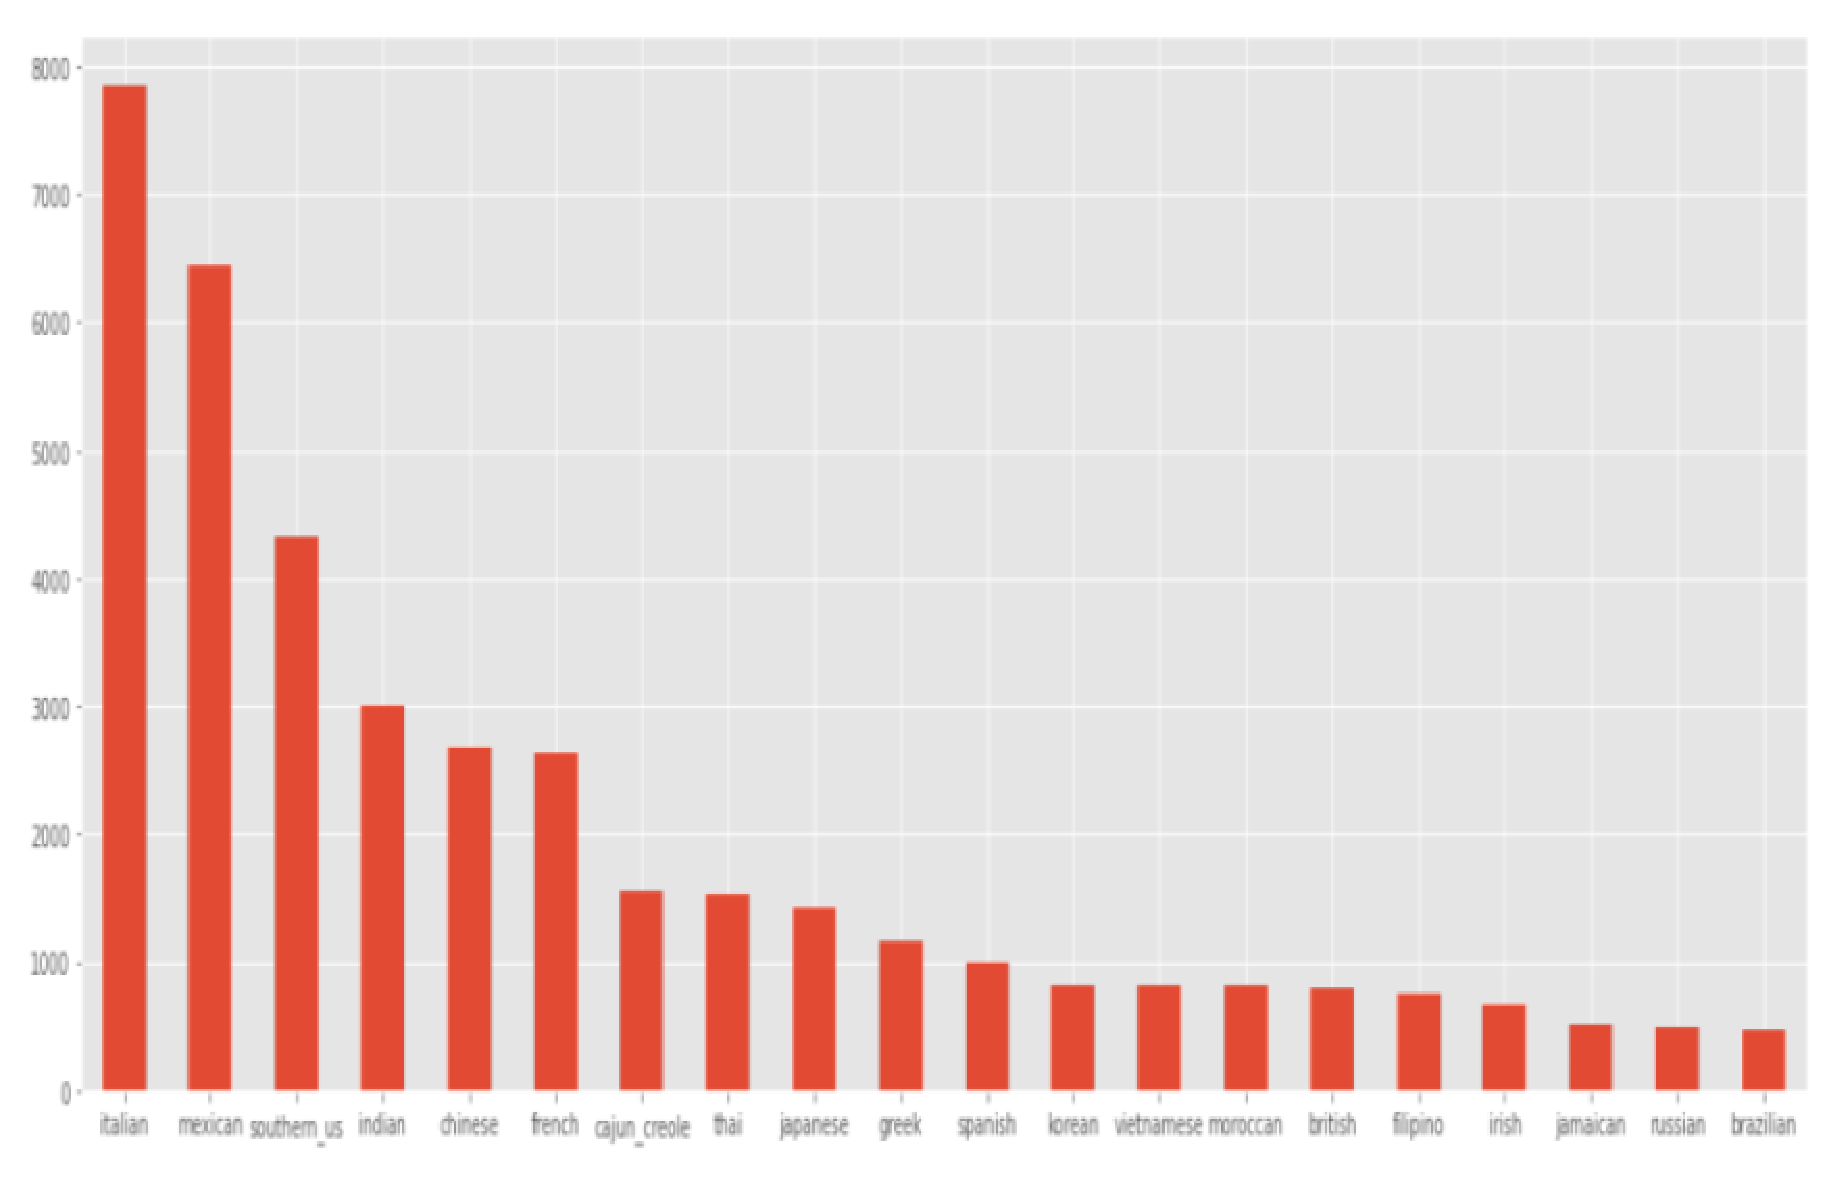
\includegraphics[width=0.6\textwidth,natwidth=866,natheight=550]{figures/ns.eps}
        \caption{number of receipes by cuisine}\label{Checking for outliers}
      \end{figure}
      
      %%==========================================================================================
      \begin{note}
      Last,
      we use the outlying degree to identify the specific group outlying aspects.
      
      The pseudo code of GOAM algorithm is as follows.
      The input is the group data,
      the output is outlying aspects of specific group ($G_1$).
      
      The details of the algorithm I will use an example to explain.
      \end{note}
  %%==========================================================================================
  
  \end{slide}
%%

%%
%%==========================================================================================
\begin{slide}{Ingredients in a Dish}
  \begin{itemize}
    \item
    Look at the graphs below 
    \begin{itemize}
      \item
      Ingredients in a dish distribution.
      
     
      \end{itemize}
    \end{itemize}
    
    \begin{figure}
      \centering
      \selectcolormodel{rgb}
      %\missingfigure{Testing.}
      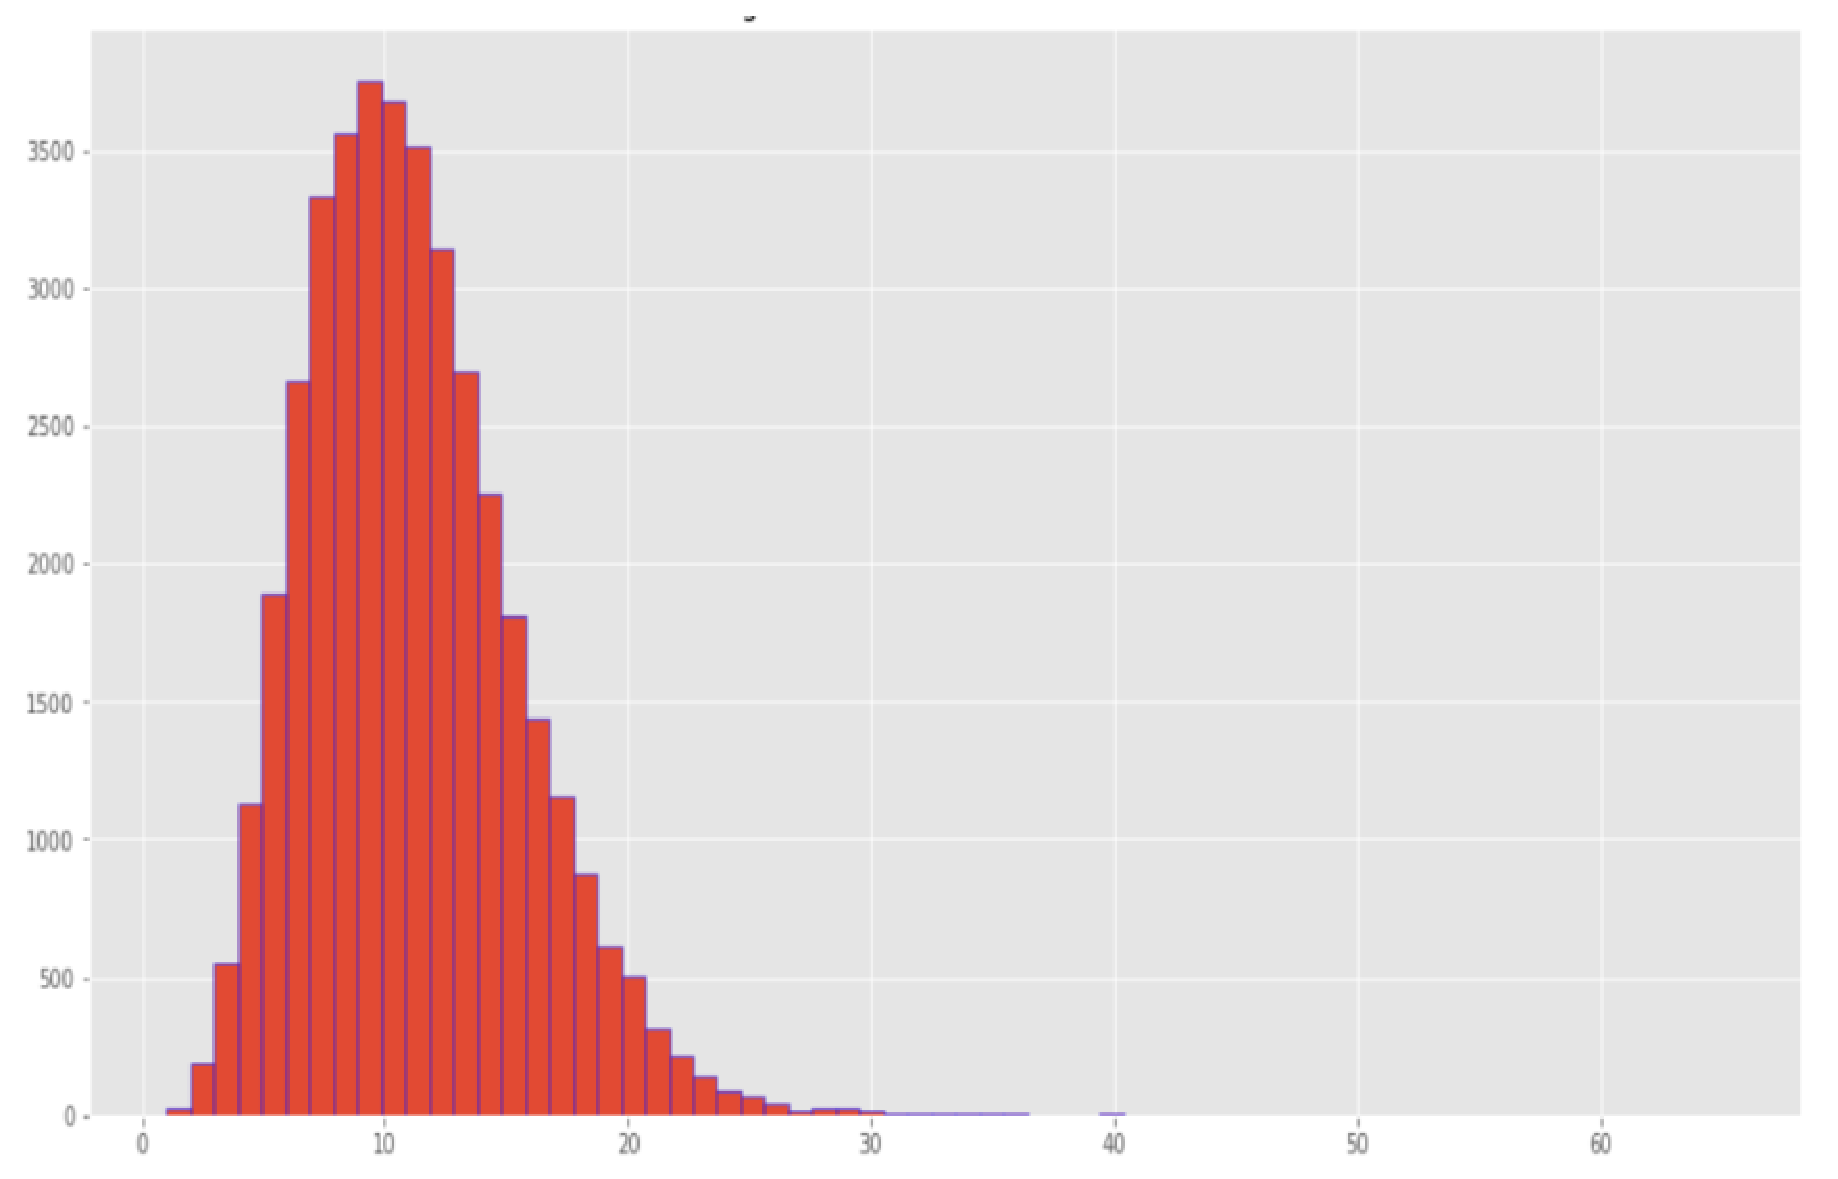
\includegraphics[width=0.6\textwidth,natwidth=866,natheight=550]{figures/cu.eps}
      \caption{distribution}\label{Checking for outliers}
    \end{figure}
    
    %%==========================================================================================
    \begin{note}
    Last,
    we use the outlying degree to identify the specific group outlying aspects.
    
    The pseudo code of GOAM algorithm is as follows.
    The input is the group data,
    the output is outlying aspects of specific group ($G_1$).
    
    The details of the algorithm I will use an example to explain.
    \end{note}
%%==========================================================================================

\end{slide}

%%==========================================================================================
\begin{slide}{Main Ingredients}
  \begin{itemize}
    \item
    Look at the graphs below 
    \begin{itemize}
      \item
      Salt is the largest share of all the Greek ingredients.
      
     
      \end{itemize}
    \end{itemize}
    
    \begin{figure}
      \centering
      \selectcolormodel{rgb}
      %\missingfigure{Testing.}
      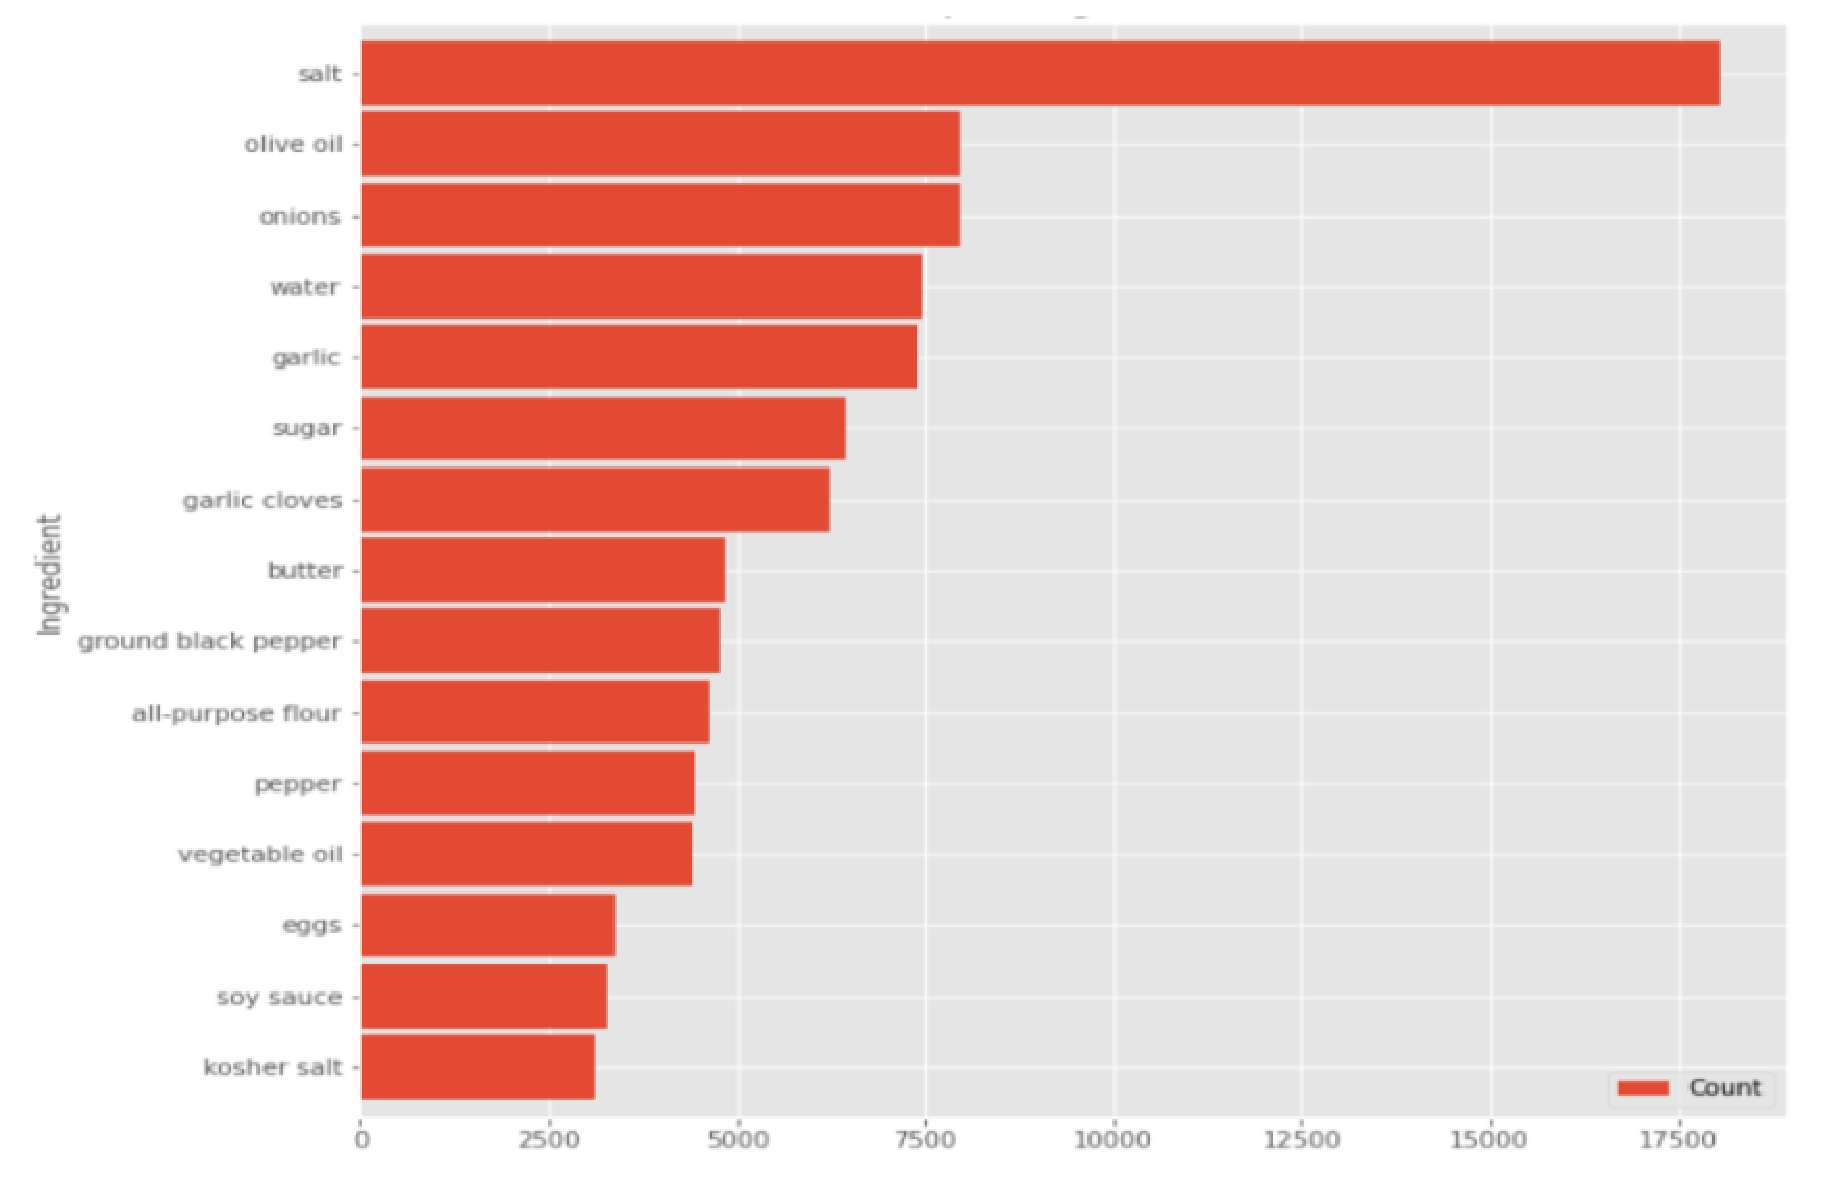
\includegraphics[width=0.6\textwidth,natwidth=866,natheight=550]{figures/15.eps}
      \caption{top 15 ingredients}\label{Checking for outliers}
    \end{figure}
    
    %%==========================================================================================
    \begin{note}
    Last,
    we use the outlying degree to identify the specific group outlying aspects.
    
    The pseudo code of GOAM algorithm is as follows.
    The input is the group data,
    the output is outlying aspects of specific group ($G_1$).
    
    The details of the algorithm I will use an example to explain.
    \end{note}
%%==========================================================================================

\end{slide}
%%%%%%%%%
\begin{slide}[toc=,bm=]{Ingredients in Each Cuisine}
  \twocolumn
  {
    
  \begin{itemize}
  \item
  \smallskip
  The proportion of ingredients in Mexican cuision.

 \end{itemize}
  \vspace{0.4cm}
  %\vspace{0.1cm}
  \begin{figure}
    \centering
    \selectcolormodel{rgb}
    %\missingfigure{Testing.}
    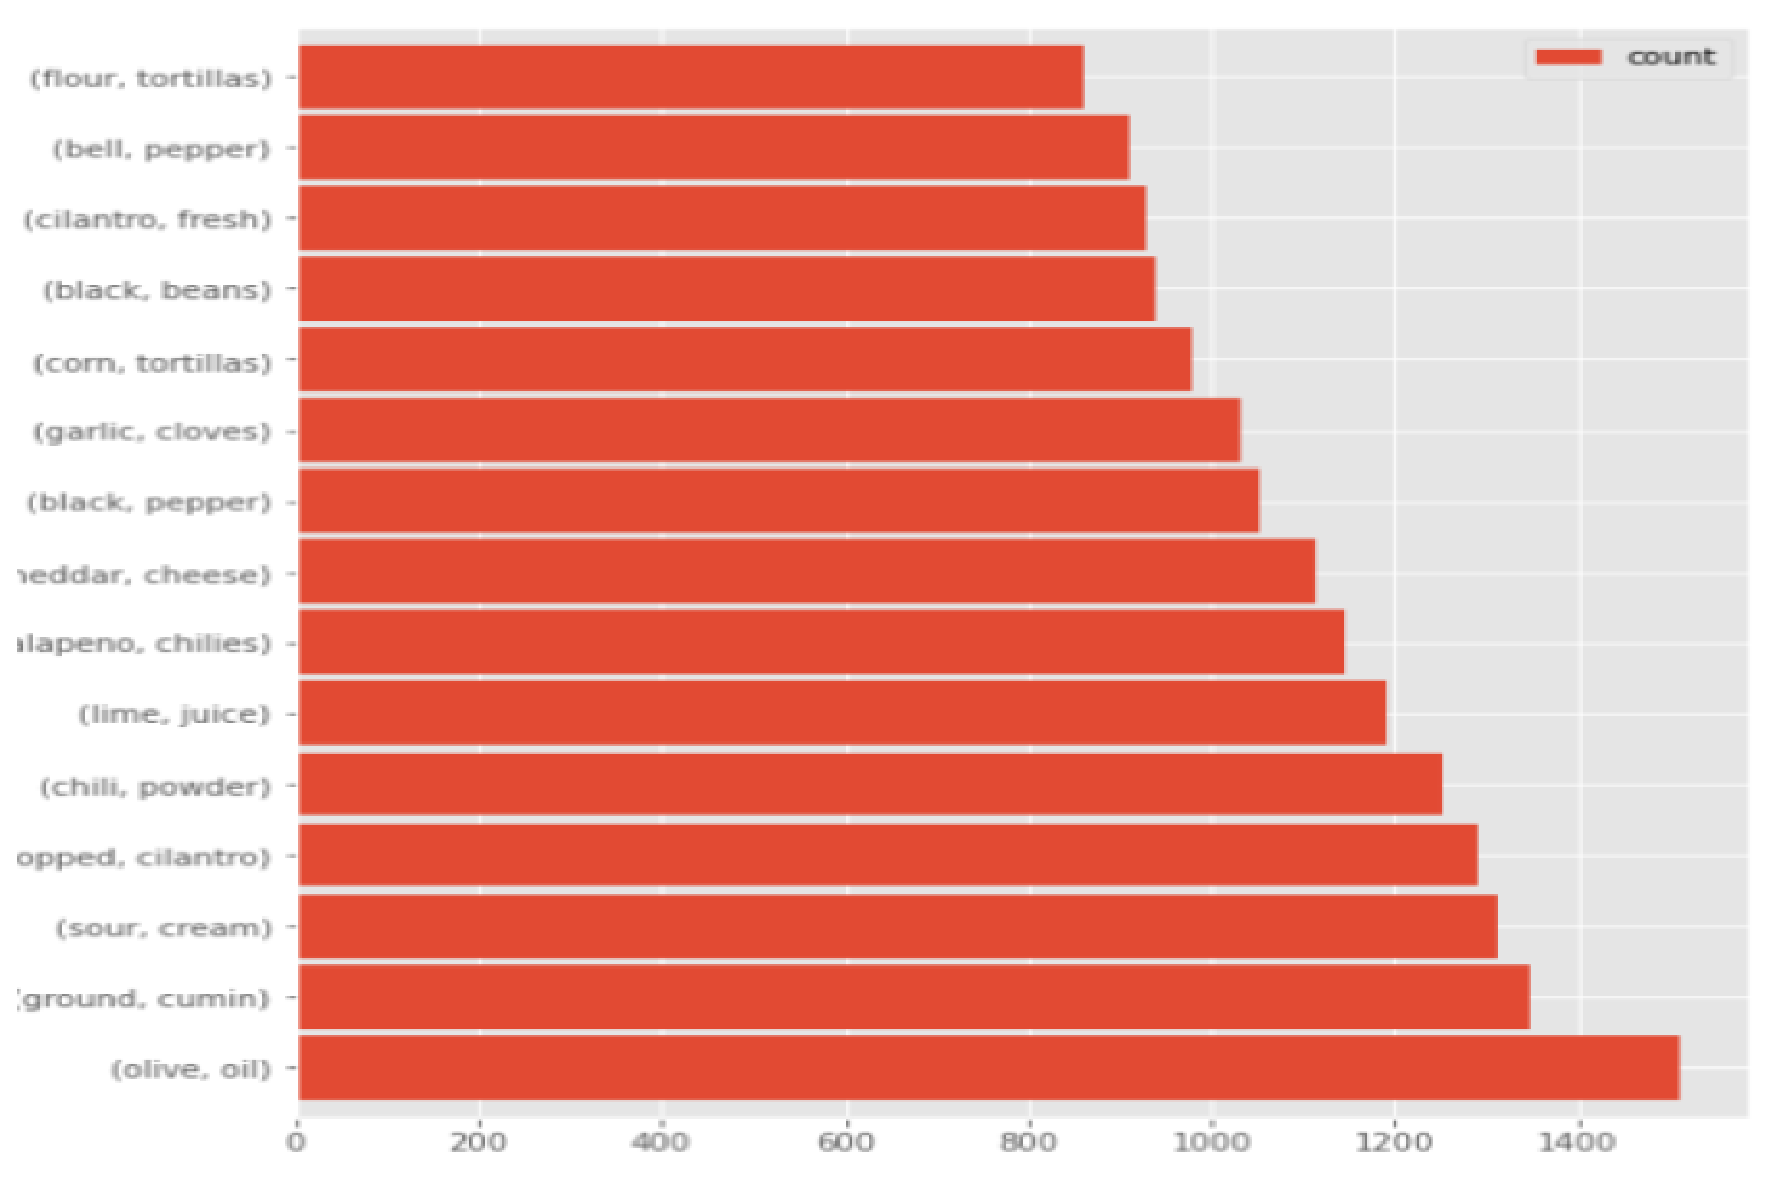
\includegraphics[width=1.0\textwidth,natwidth=840,natheight=550]{figures/me.eps}
    \caption{Mexican cuisine}\label{Checking for outliers}
  \end{figure}
  }
  {
  
  \begin{itemize}
  \item
  The proportion of ingredients in Chinese cuision.
  

  \end{itemize}
  \bigskip
  \begin{figure}
    \centering
    \selectcolormodel{rgb}
    %\missingfigure{Testing.}
    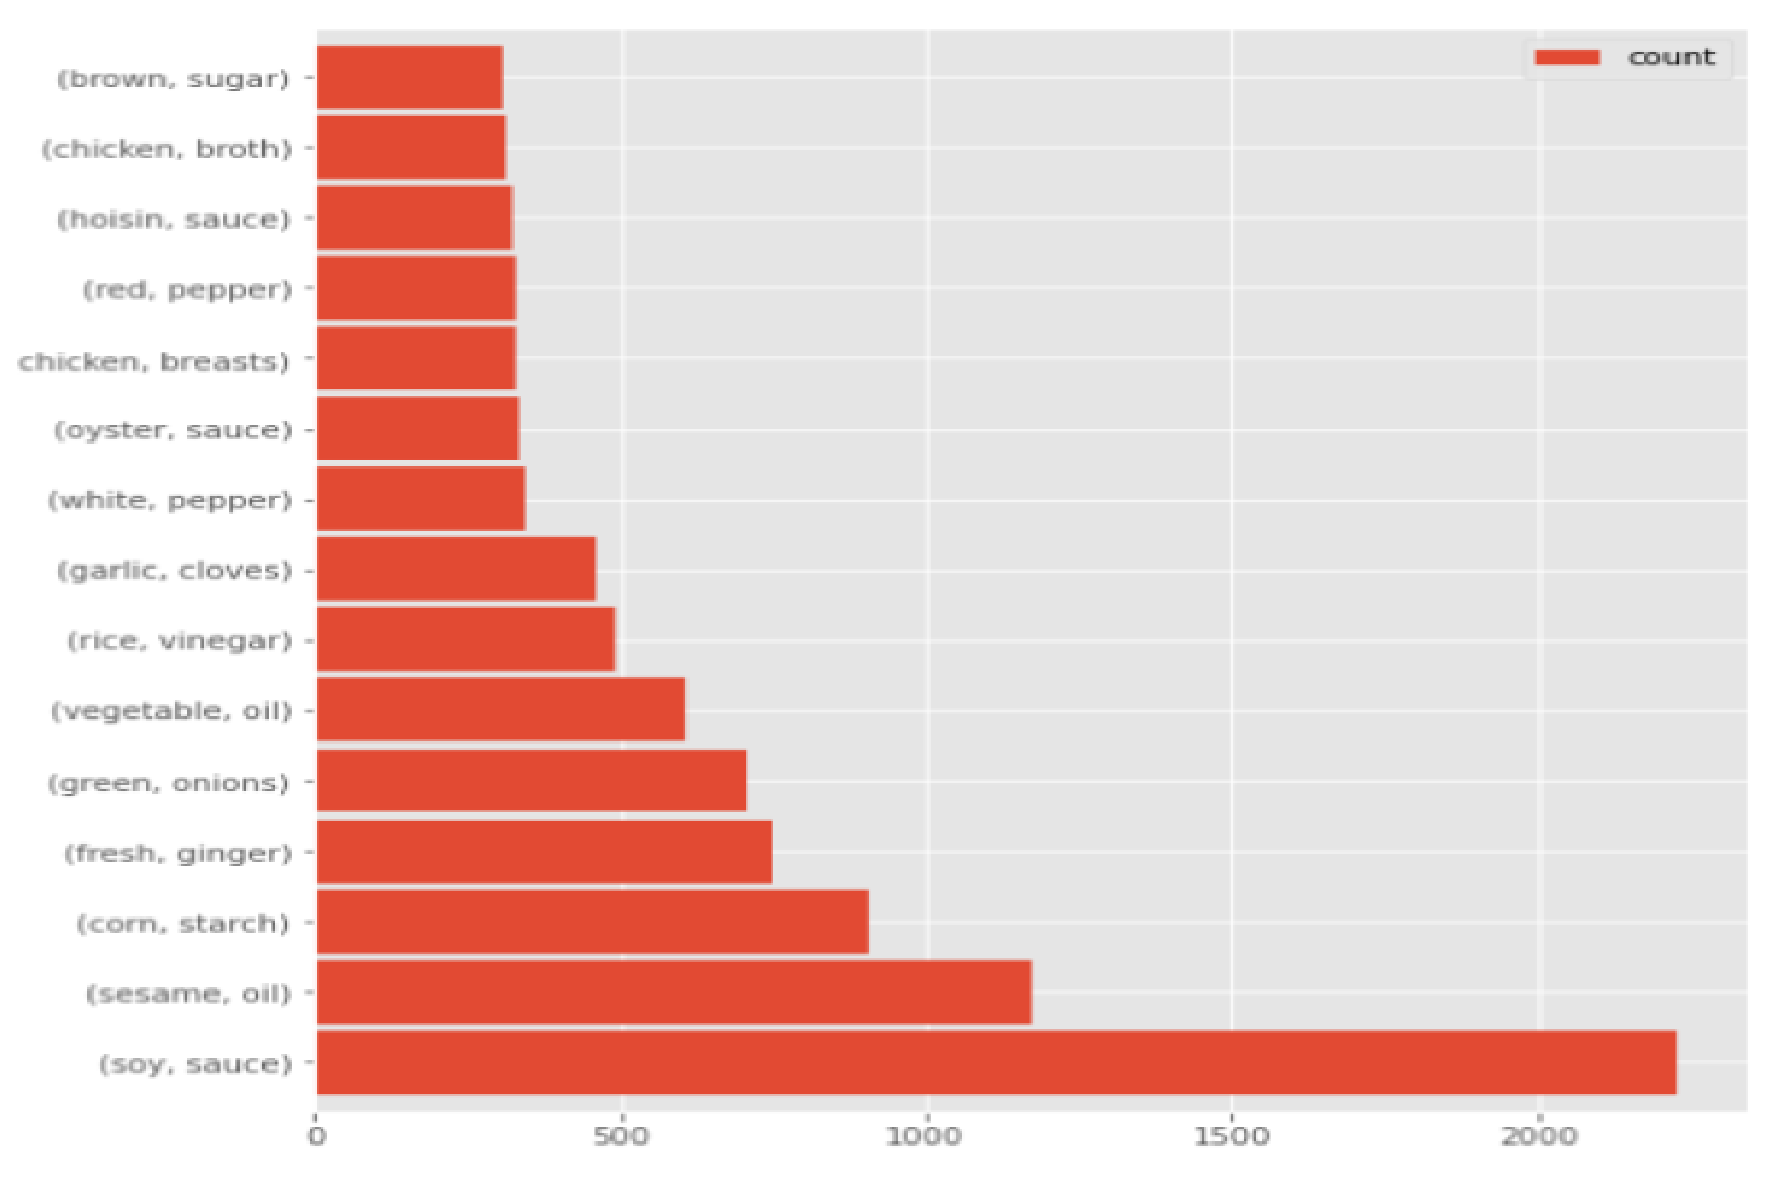
\includegraphics[width=1.0\textwidth,natwidth=840,natheight=550]{figures/ch.eps}
    \caption{Chinese cuisine}\label{Checking for outliers}
  \end{figure}
  }
  
  %%==========================================================================================
  \begin{note}
  In this research paper,
  we proposed the group outlying aspects mining.
  Now,
  let me summarize the differences between group outlying aspects mining and outlying aspects mining.
  
  Group outlying aspects mining mainly focuses on the differences between groups.
  But outlying aspects mining mainly concentrates on the differences between objects.
  The target of group outlying aspects mining can be seen as many points.
  While the target of outlying aspects mining can be regarded as one point.
  
  In the NBA example,
  group outlying aspects mining focuses on the advantages
  or disadvantages of one team,
  however,
  outlying aspects mining focuses on the advantages or disadvantages of one player.
  \end{note}
  %%==========================================================================================
  
  \end{slide}

  %%%%%%%%%%%%%%%%%%
  
%%%%%%%%%%%%%
\section{NLP Analysis}

\begin{slide}[toc=,bm=]{TF-IDF Algorithm}

  \begin{itemize}
  \item
  Model of TF-IDF algorithm
  
  \vspace{1.2cm}
  
  \begin{centering}
   
  $ TF-IDF (d, w) = TF (d, w) *IDF(w)$
  
  
  \end{centering}
  
  \begin{itemize}
  
  \item
  $TF(d,w)$ $\Leftrightarrow$ Frequency of occurrence of w in document d.
  \item
  $IDF(w) = log\frac{N}{N(w)}$
  \item
  N $\Leftrightarrow$ The total number of documents in a corpuss.
  \item
  N(w)$\Leftrightarrow$ How many documents does the w appear in.
  
  \end{itemize}
  \end{itemize}
  
  %%==========================================================================================
  \begin{note}
  Base on the earth mover distance,
  we can calculate the outlying degree using the formula shown on the screen.
  
  This formula is the outlying degree scoring function,
  n represents the number of competitive groups.
  $h_{k_s}$ is the histogram of $G_k$ in the subspace s.
  \end{note}
  %%==========================================================================================
  
  \end{slide}
%%==========================================================================================
\begin{slide}[toc=,bm=]{TfidfVectorizer Grammar}

  \begin{itemize}
  \item
  Steps.
  
  \begin{itemize}
  \item
  The counting matrix of words is converted to TF-IDF representation, and then normalized.
  \item
  Scikit-learn provides a TfidfVectorizer class, which has the ability to remove common stop words (like a, the, and, or).
  \item
  TF-IDF tends to filter out common words and retain important words.
  
 
  \end{itemize}
  \end{itemize}
  
  %%==========================================================================================
  \begin{note}
  The second challenge is how to evaluate the outlying degree of
  the query group between different aspects.
  
  In that case,
  we need to design a scoring function to measure the outlying degree.
  But adopting an appropriate scoring function without dimension bias still remains a problem.
  \end{note}
  %%==========================================================================================
  
  \end{slide}
%%

  %%==========================================================================================
  



%%
\section{Modeling}
\begin{slide}[toc=,bm=]{Logistic Regression and Ensemble Model}
  \begin{itemize}
  \item
  \textcolor{orange}{Logistic Regression}
  
  \begin{itemize}
  \item
  Random seeds are not fixed and generate random sequences.
  \item
  Use the logistic regression model in sklearn.
  \item
  Score:0.787711182622687.
  
  
  
  \end{itemize}
  
  \item
  \textcolor{orange}{Ensemble Model}
  
  \begin{itemize}
  \item
  Ensemble in Sklearn is called to integrate the two classifiers, logistic regression and SVM.
  
  \item 
  in the way of soft voting, to show the accuracy
  \item   
  Score:0.8119469026548672.  
\end{itemize}
  
  \end{itemize}
  
  %%==========================================================================================
  \begin{note}
  In terms of the strengths of GOAM algorithm.
  
  I would like to talk about two main advantages of this algorithm.
  First is the reduction of complexity.
  GOAM algorithm utilizes the bottom up search method;
  what's more,
  it can reduce the size of candidate subspaces.
  
  Second is efficiency.
  The previous time complexity is O($2^d$);
  however,
  current time complexity if only O($d*n^2$).
  \end{note}
  %%==========================================================================================
  
  \end{slide}
%%
%%==========================================================================================

  %%==========================================================================================
  

  \begin{slide}[toc=,bm=]{Create Submission}

    \begin{table}[tb]
    \setlength{\abovecaptionskip}{0pt}
    \setlength{\belowcaptionskip}{10pt}
    \centering
    \caption{Predictions from first level models}
    
    \begin{tabular}{ c | c | c }
    \toprule
      % after \\: \hline or \cline{col1-col2} \cline{col3-col4} ...
          &  ID    & Cuisine \\
    \midrule
    0 &  18009    &  british  \\
    
    1 &  28583    &  southern_us \\
    
    2 &   41580    &  italian \\
    3 &   29752    &  cajun_creole \\
    4 &   35687    &  italian    \\
    5 &   38527    &  southern_us\\
    \bottomrule
    \end{tabular}
    \end{table}
    
    %%==========================================================================================
    \begin{note}
    From table $6$,
    we can see that GOAM method can identify the trivial outlying features
    and non-trivial outlying subspaces accurately and
    it is obvious from the table that the accuracy of GOAM is the best,
    which is 100\%.
    
    This is because the outlying aspects mining method
    can't obtain the features of a group and the scoring function
    is based on point to point metric.
    Therefore,
    it is not suitable for group outlying aspects mining.
    \end{note}
    %%==========================================================================================
    
    \end{slide}
    %%
    %%==========================================================================================
\begin{slide}[toc=,bm=]{Reflection and Summary}

\begin{center}
\begin{itemize}

\item
\smallskip
\large
{Dishes can contain a variety of ingredients, and the same ingredients may vary in number and number, so the integredients need to be filtered.
  \item 
  KNN mainly depends on the surrounding limited adjacent samples, rather than on the method of discriminating class domain to determine the category.\\

\item
KNN basically does not learn, resulting in a slower prediction speed than logistic regression and other algorithms.
}

\end{itemize}
\end{center}
\end{slide}


%%==========================================================================================
%%


%%==========================================================================================
% TODO: Contact Page
\begin{wideslide}[toc=,bm=]{Contact Information}
\centering
\vspace{\stretch{1}}
\twocolumn[
lcolwidth=0.35\linewidth,
rcolwidth=0.65\linewidth
]
{
% \centerline{\includegraphics[scale=.2]{tulip-logo.eps}}
}
{
\vspace{\stretch{1}}
Thank you for listening!\\
Siyu Chen\\
Xi'an Shiyou University\\
\begin{description}
 \item[\textcolor{orange}{\faEnvelope}] \href{mailto:785987165@qq.com}
 {\textsc{\footnotesize{785987165@qq.com}}}

 
\end{description}
}
\vspace{\stretch{1}}
\end{wideslide}

\end{document}

\endinput
